%%%%%%%%%%%%%%%%%%%%%%%%%%%%%%%%%%%%%%%%%%%%%%%%%%%%%%%%%%%%%%%%%%%%%%%%%%%%%%%%
%2345678901234567890123456789012345678901234567890123456789012345678901234567890
%        1         2         3         4         5         6         7         8

\documentclass[letterpaper, 10 pt, conference]{ieeeconf}  % Comment this line out
%\documentclass[a4paper, 10pt, conference]{ieeeconf}
%\usepackage{subcaption}
\usepackage{graphicx}
\usepackage{multicol}
\usepackage{makecell}
\usepackage{lipsum}% http://ctan.org/pkg/lipsum                                                      % if you need a4paper
%\documentclass[a4paper, 10pt, conference]{ieeeconf}      % Use this line for a4
                                                          % paper

\IEEEoverridecommandlockouts                              % This command is only
                                                          % needed if you want to
                                                          % use the \thanks command
\overrideIEEEmargins
% See the \addtolength command later in the file to balance the column lengths
% on the last page of the document



% The following packages can be found on http:\\www.ctan.org
%\usepackage{graphics} % for pdf, bitmapped graphics files
%\usepackage{epsfig} % for postscript graphics files
%\usepackage{mathptmx} % assumes new font selection scheme installed
%\usepackage{times} % assumes new font selection scheme installed
%\usepackage{amsmath} % assumes amsmath package installed
%\usepackage{amssymb}  % assumes amsmath package installed
\usepackage{mdframed}
\usepackage{ntheorem}
\usepackage{subfig}
\usepackage{graphicx}
\usepackage{framed}
\title{\LARGE \bf
Predicting the Programming Language of Code Snippets Using Natural Language Processing
}

%\author{ \parbox{3 in}{\centering Huibert Kwakernaak*
%         \thanks{*Use the $\backslash$thanks command to put information here}\\
%         Faculty of Electrical Engineering, Mathematics and Computer Science\\
%         University of Twente\\
%         7500 AE Enschede, The Netherlands\\
%         {\tt\small h.kwakernaak@autsubmit.com}}
%         \hspace*{ 0.5 in}
%         \parbox{3 in}{ \centering Pradeep Misra**
%         \thanks{**The footnote marks may be inserted manually}\\
%        Department of Electrical Engineering \\
%         Wright State University\\
%         Dayton, OH 45435, USA\\
%         {\tt\small pmisra@cs.wright.edu}}
% * <kamel@uvic.ca> 2017-12-15T23:17:23.178Z:
%
% ^.
%}

%\author{Kamel Alreshedy, Dhanush Dharmaretnam, Daniel M. German, Venkatesh Srinivasan and Aaron T. Gulliver\\
%Department of Computer Science,
%University of Victoria\\
%PO Box 1700, STN CSC, Victoria BC, Canada V8W 2Y2\\
%Kamel, Dhanushd, dmg, srinivas@uvic.ca, agullive@ece.uvic.ca}


\begin{document}



\maketitle
\thispagestyle{empty}
\pagestyle{empty}
\theoremseparator{.}
\newmdtheoremenv{theo}{RQ}
\newmdtheoremenv{res}{RQ}
\newmdtheoremenv{box1}{}
%%%%%%%%%%%%%%%%%%%%%%%%%%%%%%%%%%%%%%%%%%%%%%%%%%%%%%%%%%%%%%%%%%%%%%%%%%%%%%%%
\begin{abstract} %Rewrite
 
Predicting programming languages from code snippets and textual data is a challenging task. Online forums like Stack Overflow and code repositories such as GitHub rely on accurate language tags to connect the knowledge seekers to knowledge providers. In this paper, we combine ideas from the fields of Natural Language processing and machine learning to predict programming languages for any data consisting of code snippet and text. Our classifier achieves an accuracy of 84\% in predicting the top 24 programming languages by combining features from code snippets and textual information. Our results show that using machine Learning techniques on combination of textual and code features gives better performance than using text or code features individually. Unlike other black box machine learning approaches, we conduct an extensive study of our feature spaces to identify the similarities and differences among programming languages. We also evaluated and compared our results with a paid API service- 'Programming Language Identification' tool by the Algorithmia market place which is shown to predict languages directly from source code with an accuracy of 62.8\% across 20 languages.

\bigbreak

 
\end{abstract}

\begin{keywords}
Stack Overflow, Machine learning, Programming Languages, Natural Language Processing and Algorithmia.
\end{keywords}
%%%%%%%%%%%%%%%%%%%%%%%%%%%%%%%%%%%%%%%%%%%%%%%%%%%%%%%%%%%%%%%%%%%%%%%%%%%%%%%%
 
\section{INTRODUCTION}
 
Traditionally, software projects rely on experienced programmers, code documentation and textbooks to understand the features and functionalities of a programming language. In the last decade, the advent of social media forums for programmers such as Stack Overflow, Quora and Hackers News have made learning and coding much simpler and faster. Young inexperienced developers, instead of waiting for experts in their projects, can rely on social forums to help debug their code or to implement some esoteric functionalities/libraries in programming languages. 
 
Along with the growth of online social forums for programming, the complexity and the features supported by various programming languages have also increased over the last decade due to easy access to documentation and the growth of open source repositories such as Git Hub, which enable easy access of source code of new libraries. In addition, there has been also an increased adaptation of esoteric languages such as Haskell and Scala, genesis of new languages based on existing languages such as Typescript (from JavaScript),Hack (from Php), Julia (from Matlab, C and Fortan) etc. and also splitting of languages based on standards such as  C++11, C++14, C++17 standards for C++, Java7, Java8, Java-EE6, Java9 standards for Java.
 
% 
To help developers handle this increased complexity, forums like Stack Overflow rely on the tags of questions to match them to other experienced users who can provide answers for them. However, new users in Stack Overflow or novice developers may not tag the posts correctly. This leads to posts being down voted and flagged by moderators even though the question may be important and add value to the community. This problem can be solved if the posts are automatically tagged, especially for programming languages. This motivates the main question we address in this work: {\em Can we predict programming languages from code snippets and textual data?}
 
Existing solutions to this problem are not satisfactory. Integrated Development Environment (IDE) such as Clion, Eclipse, and text editors such as notepad++, SublimeText, Atom, predict the language based on file extension rather than the source code itself. This can cause inconvenience to the users as they need to create the file with correct extension manually to enable syntax highlighting in these editors. In \cite{c18}, the authors built a classifier to predict the programming language tags in Stack OverFlow. 1000 posts were extracted to train and evaluate the model across 18 programming languages. Support Vector Machine algorithm was used to train the model. However, the method only achieves 60\% accuracy and does not work well on small code snippets.
 
There are other tools available such as Linguist by GitHub, Programming Language Identification (PLI)\footnote[1]{In the rest of this paper, PLI stands for the Programming Language Identification tool that provided by Algorithmia} tool by Algorithmia (an AI market) which predict programming language based on code snippets \cite{c12}. It is claimed that PLI tool can currently predict 20 languages with a reported accuracy of 99.4\% top1 accuracy on GitHub code snippets. However, these tools are trained on complete source code files or library files such as one from GitHub. Therefore, these tools perform better on large source code files and libraries compared to small snippets of code that are in Stack Overflow and other software forums. This leads us to first question.

 
\begin{theo}
\textbf{Can we predict the programming language using only code snippets embedded in a Stack Overflow post?}
\end{theo}
 

In this work, we will aim to devise a method for tag prediction that also works relatively well for short code snippets. While studying tag prediction from code snippets, we will also study how the number of lines of code impact the prediction capability of tools which predict programming languages from code snippets. So far, we have discussed predicting languages from code snippets. There are enormous textual data available about programming languages, its libraries and functionalities. Examples include websites like GitHub, Jira, BugZilla, Stack Overflow, Quora etc. The study of these repositories can help us to understand the programming languages, its origin and complexities. For example, mining the documentation in GitHub repositories will enable us to study the evolution of programming languages or adaptation of features and functionalities of languages. Stack Overflow posts are another source of information about programming languages. The post description texts could be mined to further enhance our understanding of programming languages and could be useful to predict the languages without using the source code. This leads us to ask the following.

 
\begin{theo}
\textbf{Can we predict the programming language by analyzing only the text describing a Stack Overflow question?}
\end{theo}
 

Recent advances in the field of machine learning, deep learning and natural language processing~\cite{c13} have resulted in an improved performance in document classification, machine translation and other predictive tasks. Therefore, machine learning and NLP techniques in immense potential in predicting the programming language from textual data. For example, it is conceivable that we can obtain word representation of the code snippet that can be combined with textual representation to further improve our prediction. This leads us to our final research question.

 
\begin{theo}
\textbf{Can we improve the prediction of programming language by analyzing both the text and code snippet information inside a Stack Overflow question?}
\end{theo}
 

The main contributions of our paper are: 
\begin{enumerate}
\item
A prediction model, based on Random Forest and XGBoost classifier, that predicts programming language tags using only the code snippet and obtains 61.5\% accuracy score.
\item
A classifier that uses only textual information embedded in Stack OverFlow posts to predict the programming language tags to achieve an accuracy score of 81.04\%, much higher than the previous model.
\item 
A third prediction method that uses a combination of code snippets and textual information available in a Stack Overflow question in order to improve its accuracy and achieves a highest score of 84.3\%.
\item 
A detailed study of the features used in our machine learning models through their projection into a 300 dimensional vectors space using Word2Vec.
\end{enumerate}

\section{Background and Related Work} % Not completed
As described in the introduction, the problem of predicting the programming language from dataset posts consisting of a text and code snippets is a topic of immense interest to the computer science research community. Despite this, our understanding of this topic is very poor.
 
The only previous published work on this topic, to the only best of our knowledge, is the work of Baquero {et al.}~\cite{c18}. They extracted a set of 18000 question posts from Stack OverFlow that contained text and code snippets, 1000 posts each for 18 programming languages. They evaluated their classifier, trained using Support Vector Machine model, on text features and source code features. They achieved an accuracy of 60\% for text features and 44\% for code snippet features. Another contribution of their work the use of feature representation to visualize the relationship between the programming languages and identify those that are closely related.
 
Algorithmia is a popular online market place which enabled use of machine learning models as a micro service using REST API. ProgrammingLanguageIdentification (PLI) is one among many tools hosted by Algorithmia and currently supports 21 programming languages. The approximate cost for making 10,000 API calls to PLI is 20 USD. The tool was originally trained using source code from various GitHub repositories and claims 99.4\% accuracy. Since Algorithmia is the only well known tool for predicting language from code snippets, we compare our method with Algorithmia.
 
As related examples, some editors (Sublime, Atom) provide some interesting highlights to code on the basis of programming language. However, they require explicit mention of the extension (eg .html, .css, .py and so on). Along similar lines, Portfolio \cite{c6} is a search engine that supports programmers in finding functions that implement high level requirements in query terms. This search engine does not identify the coding language. However, it analyzes code snippet and extracts valuable functions which can be reused. Another tool developed by Holmes \textit{et al.} \cite{c8} called Strathcona can find similar snippets of code.
 
To understand the factors that differentiate a good post from a bad post, Nachi \textit{et al.} \cite{c3} studied what makes a post good or bad based on lines of code, quality of code and texts in a Stack Overflow post. Similarly, C. Treude \textit{et al.} \cite{c5} analyzed Stack OverFlow questions to explore the type of questions that receive a good answer. They found that the posts which contained snippets of code receive a good answer. 
 
Software maintainers prefer to talk to each other to understand the code~\cite{c9}. Researchers found three reasons why the programmers use Q\&A web site: just-in-time learning, clarifying their knowledge and remembering the details. Programmers generally use the web as the main source to gather information and find a solution for their problem~\cite{c4}. They use code, documentation and links to ask their questions in online forums. This gives us opportunity to use both code and text to study and learn programming languages and also to predict them from these data sources.
Rekha \textit{et al.}~\cite{c10} proposed a hybrid auto-system tagging system, that suggests a tag for the user after entering the question. Saha~\textit{et al.}~\cite{c1} followed the approach of converting Stack Overflow questions into vectors, and then training Support Vector Machines on the basis of those vectors and eventually suggesting tags on the basis of built model. The accuracy for tag prediction for their model ranged from 50\% to 100\%. Although their tagging system works efficiently for some specific tags, it does not work well with some basic tags, like Java. Another suggestion by Stanley and Byrne~\cite{c2} is to use a cognitively-inspired Bayesian probabilistic model. Their approach is to choose one most suitable tag for each post, the tag with highest log odds of correctness when each tag's prior probability is known. However, their model normalizes the top activations for all posts. So it is unable to differentiate between a post where the top predicted tag is certain, and a post where the top predicted tad is questionable. This model is 65\% accurate when asked to predict one tag per post on the average. In summary, most of the prior work falls short of creating a robust system which can assign tags to programming languages.

\section{Dataset extraction and processing}
 
In this section we discuss in detail about why Stack Overflow was chosen as the ground truth dataset for our study, how the data from Stack Overflow dump was extracted, and how the data was processed to answer our research questions. 

\subsection{Why did we select Stack Overflow as ground truth dataset for our proposed study?}
Stack Overflow is a question and answer online forum for software developer community. Developers post questions on various coding, implementation, and debugging aspects of programming. These questions are then answered by experts in various domains. According to Quantcast~\cite{c17}, a popular web traffic analytics website, Stack Overflow had 2.9 Billion global visits and 7.3 Billion global views between Dec 15, 2016 and Dec 14, 2017. Stack Overflow is the most popular forum among the developers with 1.2 million unique visits to the page between Nov 23, 2016 and Dec 14, 2017. 

As of July 2017, Stack Overflow had 37.21 million posts, among which 14.45 million are question posts, and 50906 unique tags. However, around 87\% of the Stack Overflow posts are related to 150 tags. Thus, most of the Stack Overflow tags are not that popular or are relatively new. However, in this paper, the programming language tags in the Stack Overflow are of interest. The most popular 24 programming languages as per the 2017 Stack Overflow developer survey were selected for our analysis ~\cite{c22}. They constituted about 93\% of questions in Stack Overflow. Even though the rest of 7\% tags were also related to some programming languages, they lacked a language tag. For example, Pandas is a popular library in Python for reading large Comma-Separated Values (CSV) files. The questions associated with Pandas do not have the Python tags. This could create confusion among developers who may be new to a programming language and are not familiar with all of its popular libraries. The problem of missing language tags could be addressed if posts are automatically tagged with their associated programming languages. The languages that were selected for our study are listed below: 

\begin{framed}
Assembly, C, C\#, C++, CoffeeScript, Go, Groovy, Haskell, Java,  JavaScript, Lua, Matlab, Objective-c, Perl, Php, Python, R, Ruby, Scala, Sql, Swift, Typescript, Vb.net ,Vba
\end{framed}

\subsection{How did we extract and process the data from Stack Overflow?}
The Stack overflow July 2017 data dump was used for all our analysis. The Stack Exchange Data dump for Stack OverFlow was downloaded in .xml from archive.org. 10000 question posts was selected for each programming language posted in Stack Overflow between the period of 2012 to 2016. Each post had a score of greater than 1. This was done to ensure that these posts have been in the Stack Overflow for a longer period of time and have been properly reviewed and tagged as required by the standards of the forum. The score of more than one ensure that its a good quality post. However, we were able to extract 10,000 such posts for only 20 languages. Assembly (9121), Groovy (6978), Coffee Script (3918) and Lua (6149) had less than 10,000 posts which fitted our criterion for selection of posts. Fig. 2 is shown that the number of lines of code snippet in Stack Over Flow posts.


\begin{figure*}
  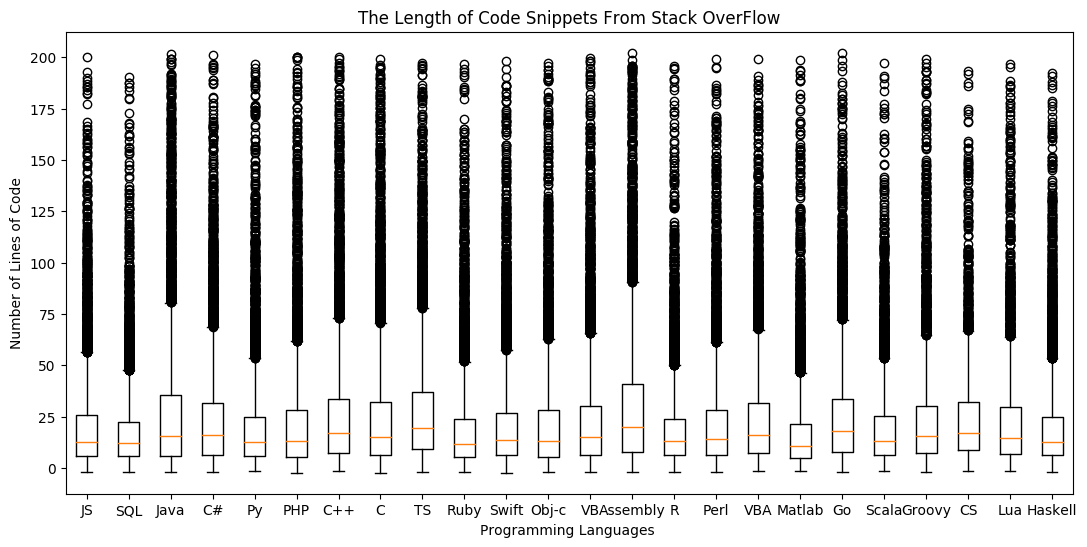
\includegraphics[width=\textwidth,height=7cm]{PlotBox.png}
  \caption{The box plot showing the number of lines of code in the extracted code snippets for all the languages. It should also be noted here that there are at least 400 posts which had more than 200 lines of code, however was not included while making this plot.}
  \label{fig:BOXPLOT}
\end{figure*}

 
The data in .xml was parsed using xmltodict and Beautiful Soup library in python to extract the code and text from the question posts separately. A Stack Overflow question post consists of a title, body and embedded code. The texts from the post were separated into three categorized namely- text (title and body of the post without code fragments), the code and code and text combined. The texts from the post (title and body) were preprocessed by removing all non English characters using Regex. After the preprocessing, they were subjected to dependency parsing using the Spacy Library. After the dependency parsing we only extracted the named entities which are nouns or noun phrases. Then, stemming and lemmatization were performed using NLTK library in python. A custom stop word dictionary was created by combining the stop words from scikit learn~\cite{c13}, Spacy~\cite{c23} and NLTK~\cite{c12} python libraries and removed these stop words. The data was then stored in separate SQL tables. This extracted vocabulary was also stored into another SQL table. Therefore at the end of this stage, we are left with a database with below 4 SQL tables.

\begin{itemize}
  \item 213,834 code snippets.
  \item 213,834 text snippets.
  \item 213,834 text snippets and code snippets combined.

\end{itemize}

In order to make our model generalize across various standards of code, we ensured that tags belonging to various language version standards were included. For example, for python, we extracted code for the tags: python-3.x, python-2.7, python-3.5, python-2.x, python-3.6, python-3.3 and python-2.6, for Java, we selected java-8 and java-7 as the tags and finally for C++, we selected c++11, c++03, c++98 and c++14 as tags. These posts were included as a part of 10,000 posts selected for each language. We also ensured that our code snippets that were selected as a part of our dataset had a large variation in terms of lines of code. We have plotted a box plot Fig\ref{fig:BOXPLOT} showing the variation of lines for the programming languages in our dataset. It may be worth noting that our dataset includes code snippets as short as 6 lines of code to large snippets of 800 lines. 
 
Evaluating and comparing the performance of our tool against Algorithmia PLI is one of the objectives of this paper. However, the 24 languages that we selected do not match with the 20 languages in Algorithmia. Therefore, we extracted data from Stack Overflow for the missing languages- Bash, HTML and CSS which are not present in our model but in Algorithmia using the same process described in Section 2. These additional three languages were never included for training or testing our models. The languages supported by Algorithmia PLI are given below:

\begin{framed}
Bash, C, C\#, C++, CSS, Haskell, HTML, Java, JavaScript, Lua, Objective-c, Perl, PHP, Python, R, Ruby, Scala, SQL, Swift, Vb.net.
\end{framed}

%talk about lines of code here and box plot.
 

\section{Methodology}
In this section we talk in detail about the methodology we followed in answering our research questions. 
  
% 1. Discuss the Algorithms used and why they were chosen
The text and code snippets extracted from the Stack Overflow posts were split using Tf-Idf vectorizer from the Scikit learn library. we set the min-df (Minimum Document Frequency) parameter to ten which means that we will only include words which are present in at least 10 documents among all available documents. This scheme helps us to remove the rare words from our dataset and this in turn reduces the noise. We left the max-df (Maximum Document Frequency) parameter to default since we have already removed the stop words in the data pre-processing step in section 3. We selected Random Forest Classifier and XGBoost which is a gradient boosting algorithm as our machine learning models. We report precision, recall, Accuracy, F score and confusion matrix as our metrics for all our classifiers in section 5.
 
% 2. Discuss how the parameters for the algorithms were tuned

The machine learning models were hyper-tuned using RandomSearchCV - A tool for parameter search in Scikit-learn. XGboost algorithm has many hyper parameters such as minimum child weight, max depth, L1 and L2 regularization, and various evaluation metrics such as Receiver Operating Characteristic (ROC), accuracy and f score. Similarly, Random Forest Classifier which is an bagging classifier has a parameter called 'no of estimators' which are subtrees used to fit the model. It therefore become really important to tune the model by varying these parameters. However, parameter tuning is computationally expensive using standard Grid Search. Therefore we adopted a technique borrowed from deep learning called Random Search hyper tuning to train our models. The parameters for all our models were fixed after performing RandomSearch on the cross validation sets (Stratified ten fold cross validation). It may be noted that the dataset was split into train and test in the ratio 80:20, where train was used for training and cross validation and test set was used to report all final metrics in this paper. The code snippet, text and code snippet + text dataset models all followed the same approach described here.
 
% 4. Write about how Algorithmia was evaluated
Our trained model was compared with Algorithmia PLI. The evaluation process was divided into two separate steps:
\begin{enumerate}
\item
Evaluation for the 20 languages supported by Algorithmia PLI.
\item Evaluation for 17 languages common to our model and Algorithmia PLI.
\end{enumerate}
We selected 75 code snippets randomly sampled from our test dataset to perform evaluation. We used the urlib library in python to make the API calls to Algorithmia PLI to get predictions for all 20 programming languages supported by it. The API call returns a JSON file with languages as key and corresponding probability for all the 20 languages. We compared the predicted language with the ground truth to generate all our metrics. Our metrics included accuracy, precision, recall and F score. We also created a confusion matrix to further evaluate our results. 
 
% 3. Write about word2Vec and Doc2Vec
Another important contribution of this paper is the study of the vocabulary and feature space used in our algorithms. A word2vec model \cite{c20} was trained on our extracted code and text datasets using Gensim- A python framework for vector space modeling \cite{c19}. The resulting model represented each word in our vocabulary in a 300 dimensional vector space. However, it is impossible to visualize concepts in such high dimensional space. Therefore, we used t-SNE \cite{c21} which is a popular dimensionality reduction algorithm to reduce the number of dimensions of our word vectors to 2. We then selected top 3\% words from our vector embeddings for each programming language and analyzed the word similarity and cosine distance. The code and text features which are closer to one another in vector space was selected for every language using cosine cosine as measurement. These features were then combined across all languages (Dictionary of named entities) and used in our machine learning models. These results are reported in results and discussion section.

\section{Results and Discussions}
\bigbreak


 
\begin{table}[t]
  \centering
  \begin{tabular}{| c | c | c | c |}
     \hline
      Programming Language & Precision & Recall  & F1-score\\ \hline
PHP&	0.89&	0.72&	0.79\\ \hline
Go	&0.9	&0.7&	0.79\\ \hline
Coffeescript&	0.88&	0.72	&0.79\\ \hline
Groovy	&0.86	&0.71	&0.78\\ \hline
Javascript	&0.91&	0.67&	0.77\\ \hline
C	&0.85	&0.7&	0.77\\ \hline
Haskell	&0.87&	0.68	&0.76\\ \hline
Swift	&0.89&	0.63	&0.74\\ \hline
Assembly&	0.83&	0.64&	0.73\\ \hline
Vba&	0.83&	0.66&	0.73\\ \hline
C++	&0.84	&0.62&	0.71\\ \hline
Matlab&	0.83	&0.59&	0.69\\ \hline
Vb.net&	0.84&	0.57	&0.68\\ \hline
Scala&	0.69&	0.66	&0.68\\ \hline
Lua&	0.83&	0.57&	0.68\\ \hline
Python&	0.85&	0.53&	0.65\\ \hline
Perl	&0.77&	0.57&	0.65\\ \hline
R	&0.72	&0.53&	0.61\\ \hline
C\#&	0.75&	0.5&	0.6\\ \hline
SQL&	0.63&	0.54&	0.59\\ \hline
Ruby&	0.62&	0.56&	0.59\\ \hline
Java&	0.64&	0.51&	0.57\\ \hline
Typescript&	0.65&	0.48&	0.55\\ \hline
Objective-c&	0.15&	0.86	&0.25\\ \hline

  \end{tabular}
  \caption{Performance Metrics for our classifier trained on code snippet features. This classifier achieves an accuracy of 62.4\% in predicting 24 languages from code snippets.}
  \label{Table:Code}
\end{table}



%first part of the section
In the first part of this section, we describe in detail the results we have obtained towards answering the following research question.

\begin{res}
Can we predict the tags of programming languages using only code snippets from the data?
\end{res}

We trained two machine learning classifiers on the code snippets extracted from Stack Overflow questions. The Random Forest and XGBoost classifier achieved an accuracy of 60.4 and 62.4\% respectively. These models were trained on the code features extracted from the code snippets using Word2Vec as described under methodology section. In this section, we will focus only on the results of XGBoost classifier which is the top performing model. The languages such as Groovy (0.78), Go (0.79), Coffee Script (0.79) and PHP (0.79) had the highest F1 Score metrics as indicated in brackets. SQL (0.59), Java (0.57), Type Script (0.55) and ruby (0.59) performed poorly. However, the worst performing programming language was Objective C with an F1 score of 0.25 with high recall of 0.86 but with poor precision of 0.15. This means that the classifier confuses Objective C with other languages. When we analyzed the code features for Objective C, we found that it shares code syntax with multiple other languages such as C, Java, Python, C++ and even C\#. There are not many unique code features available to Objective C which could enable the classifier to uniquely identify it. A small number of code features that we extracted for Java and SQL could be found under Fig\ref{fig:Java} and Fig\ref{fig:SQL} respectively.  The detailed performance metrics of our code feature based classifier could be found under table \ref{Table:Code}.



The next step was to compare our code snippet based classifier with Algorithmia PLI classifier. We performed this comparison by evaluating the results we obtained by running the prediction of programming languages using the tool from Algorithmia for 1500 snippets of code across 20 different programming languages. The tool gave an accuracy of 62.8\% in predicting languages from code snippets with an F score of 0.64. The tool has a precision of 0.68 and a Recall of 0.63. The confusion matrix for this prediction task is shown in Fig\ref{fig:AlgorithmiaConf}. We can infer from the confusion matrix that some languages such as Scala, Haskell, Ruby, Objective C and python performs much better as compared to languages languages such as HTML, CSS, JavaScript and SQL performs the worst. Scala and Haskell are not often confused with other languages due their unique syntax. It is bit surprising to us that Objective C is not confused with C language since they both have very similar syntax. It could be because objective C is much more similar to C++ than C language. This is evident from some Objective C code snippets which are confused in with languages such as Java, Ruby, Scala and C which is similar to the results from our code snippet based classifier.
 
HTML, CSS and JavaScript are used together in web development and moreover, CSS and JavaScript are often embedded in the HTML files which could explain why the tool performed very poorly in identifying these languages. We manually analyzed the Code snippets from HTML, CSS and JavaScript and found that in more than 60\% of the cases, the tool generated wrong predictions because of them being used together in the same code snippet. However, in rest of the cases the tool simply got them wrong. We speculate that this could be due to the reason that training data might have had embedded CSS and JavaScript in them which makes the tools performance on these languages much lower as compared to other languages. The poor performance of SQL could be attributed to the fact that SQL is mostly embedded in the code snippets of other programming languages such as Python, C, C++, Java etc. From the confusion matrix (Fig\ref{fig:AlgorithmiaConf} , we could see that SQL is mostly confused with Scala, Ruby and R. 




\begin{table}[t]
  \centering
  \begin{tabular}{| c | c | c | c |}
     \hline
      Programming Language & Precision & Recall  & F1-score \\ \hline
C	&0.97&	0.94	&0.96	 \\ \hline
Swift	&0.99	&0.92&	0.95	\\ \hline
Go	&0.96&	0.93	&0.95	\\ \hline
Coffeescript&	0.97	&0.93	&0.95	\\ \hline
Groovy&	0.98	&0.9	&0.94	\\ \hline
Assembly	&0.94	&0.91	&0.93\\ \hline
Haskell	&0.94&	0.92&	0.93	\\ \hline
Objective-c	&0.92	&0.92&	0.92\\ \hline
Javascript&	0.91&	0.91&	0.9\\ \hline
C++&	0.96	&0.87&	0.91\\ \hline
PHP	&0.93&	0.85&	0.89	\\ \hline
Matlab	&0.9&	0.87	&0.88\\ \hline
Perl	&0.87&	0.84	&0.86\\ \hline
Python&	0.91&	0.8&	0.85\\ \hline
Vb.net	&0.82	&0.89&	0.85\\ \hline
Scala	&0.8&	0.91&	0.85\\ \hline
Vba	&0.82	&0.84&	0.83\\ \hline	
R	&0.81&	0.82&	0.81\\ \hline	
Typescript	&0.82	&0.77	&0.8\\ \hline
Ruby	&0.74	&0.8&	0.77	\\ \hline
Lua	&0.77	&0.68&	0.72	\\ \hline
SQL&	0.6	&0.72&	0.65\\ \hline
C\#	&0.7	&0.61	&0.65\\ \hline
Java&	0.52&	0.69	&0.6	\\ \hline
  \end{tabular}
  \caption{Performance Metrics for our classifier trained on code and text features. This classifier achieves an accuracy of 84.2\% in predicting 24 languages.}
  \label{Table:COdeText}%
\end{table}
\bigbreak
\begin{figure*}[t]
  \centering
  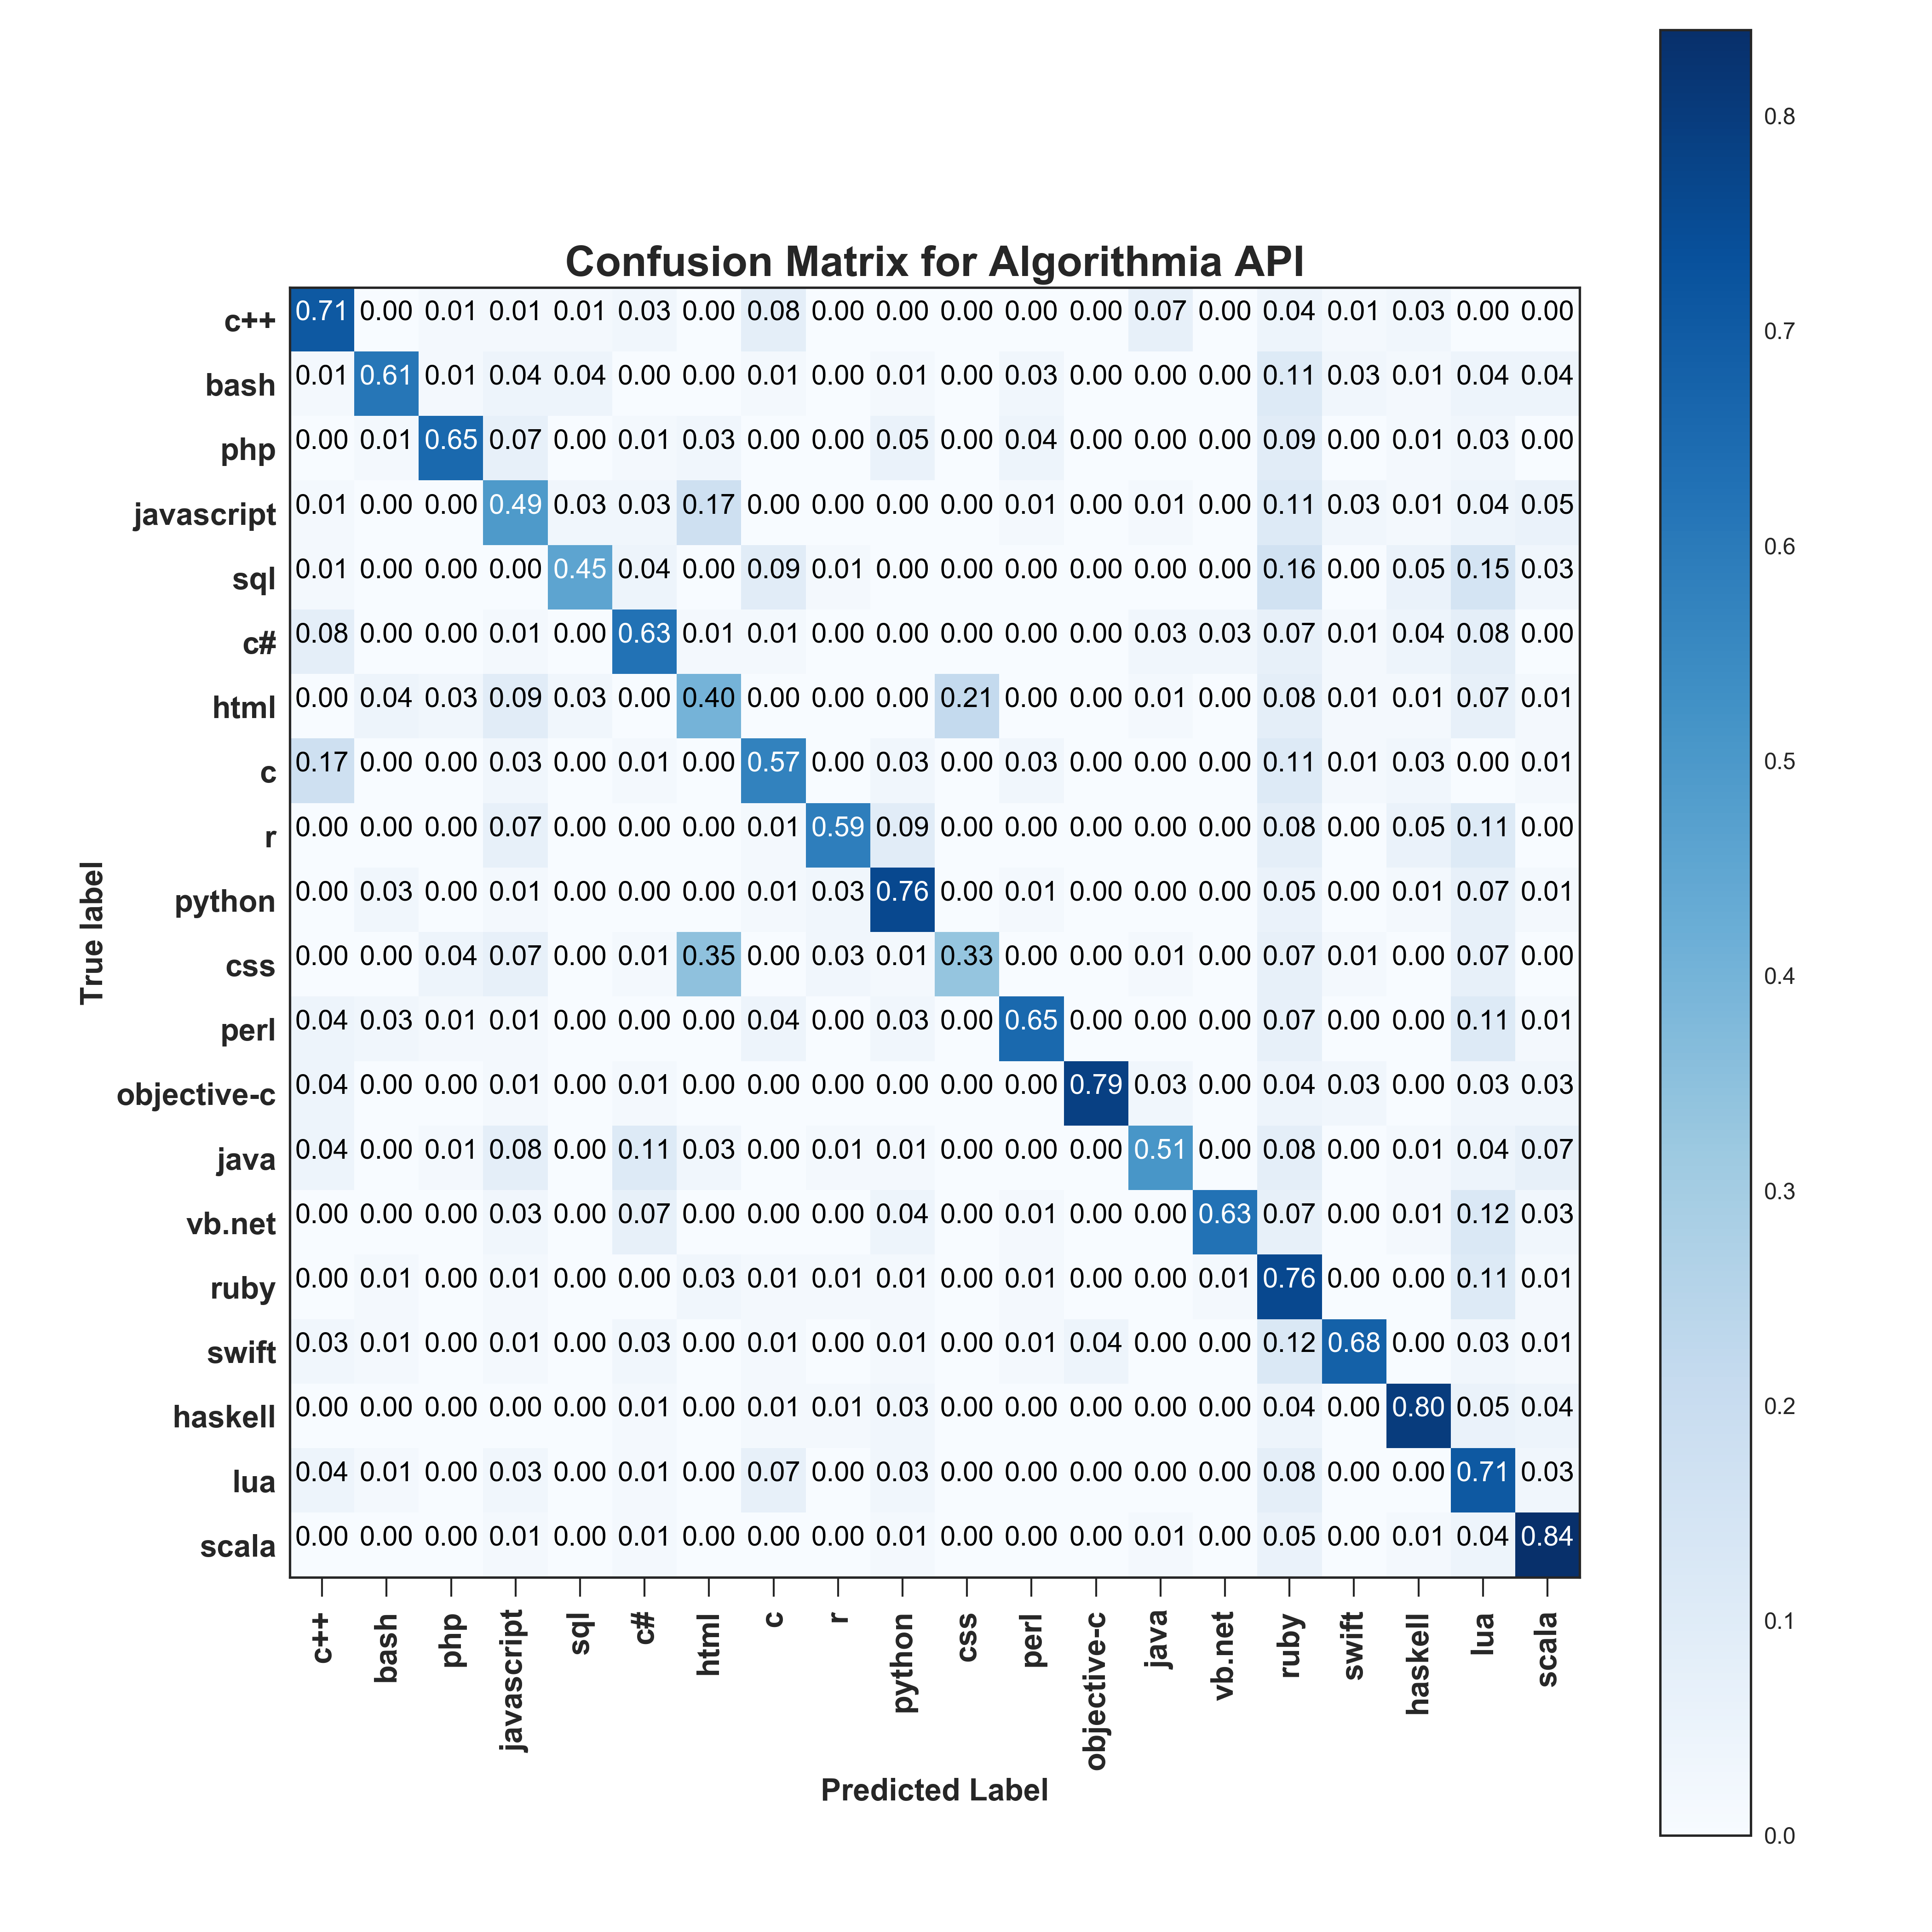
\includegraphics[width=11cm]{Fig/ConfusionMatrixAlgorithmia}
  \caption{Confusion matrix for language prediction from text using random forest classifier.}
  \label{fig:AlgorithmiaConf}
\end{figure*}

\begin{figure*}[t]
  \centering
  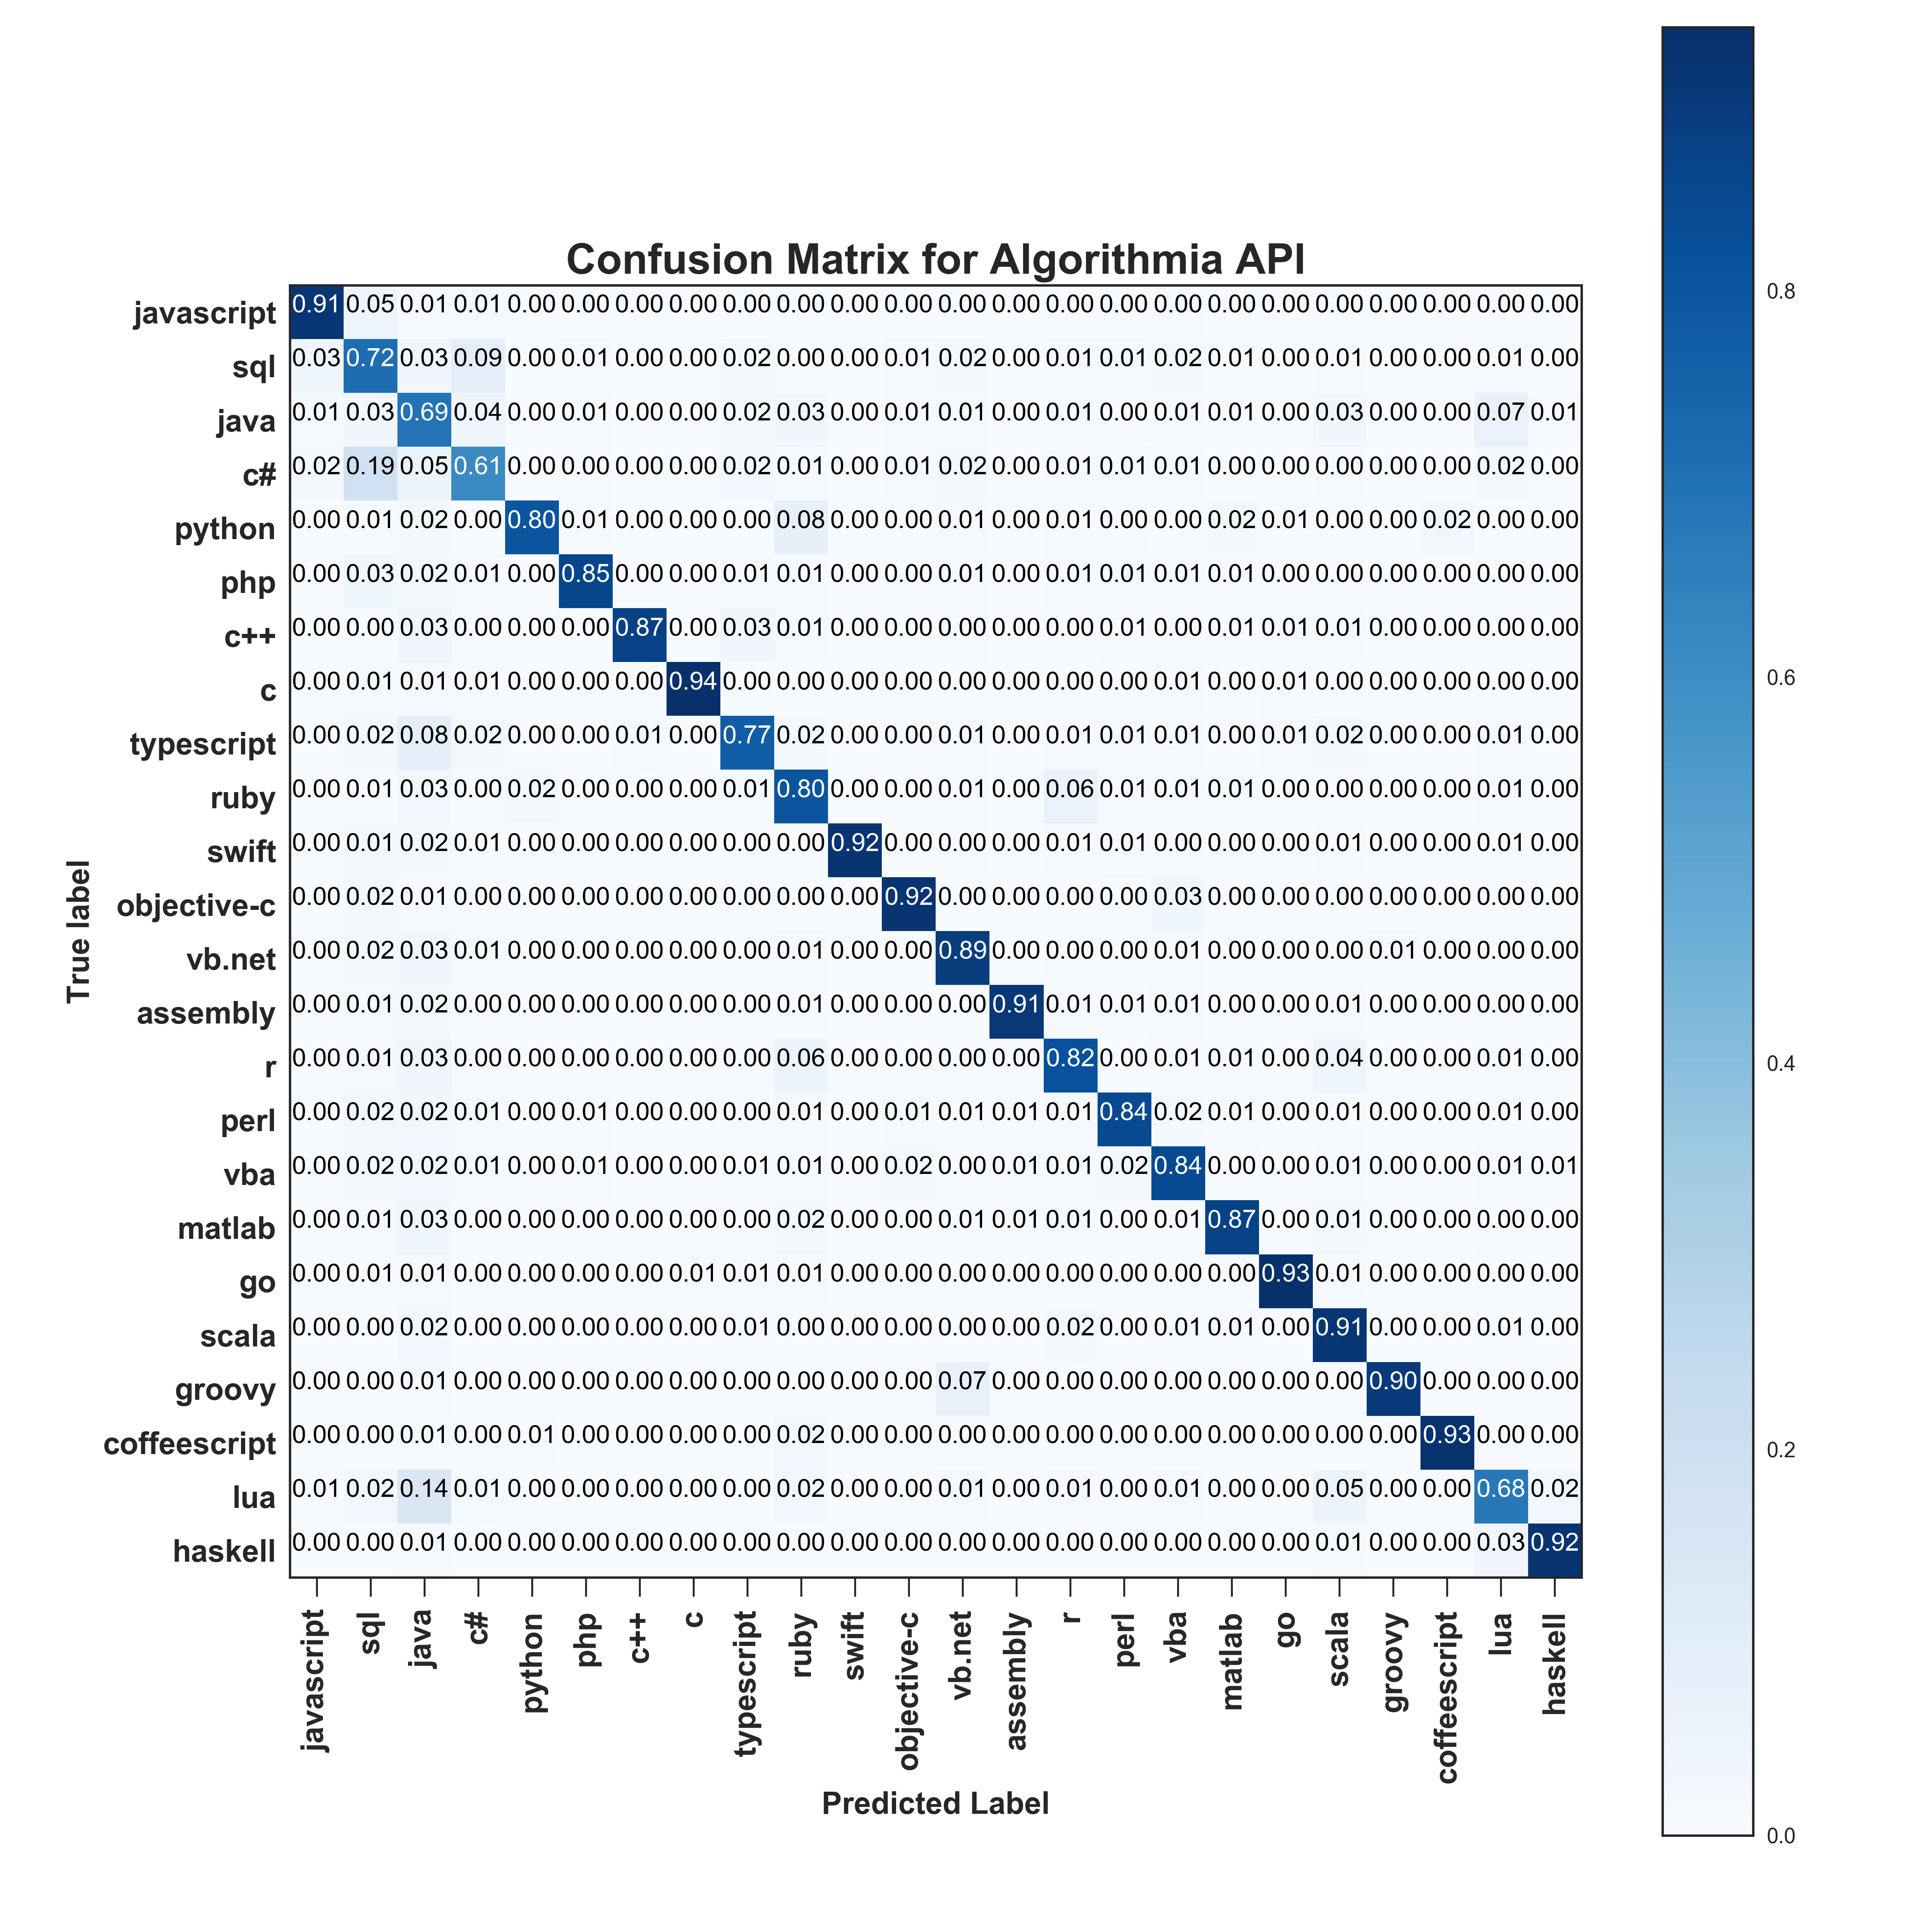
\includegraphics[width=11cm]{Fig/ConfusionMatrixOurCdeText}
  \caption{Confusion matrix for language prediction from text using random forest classifier.}
  \label{fig:CodeTextConf}
\end{figure*}

\begin{figure*}[t]
    \centering
    \subfloat[Java Code]{{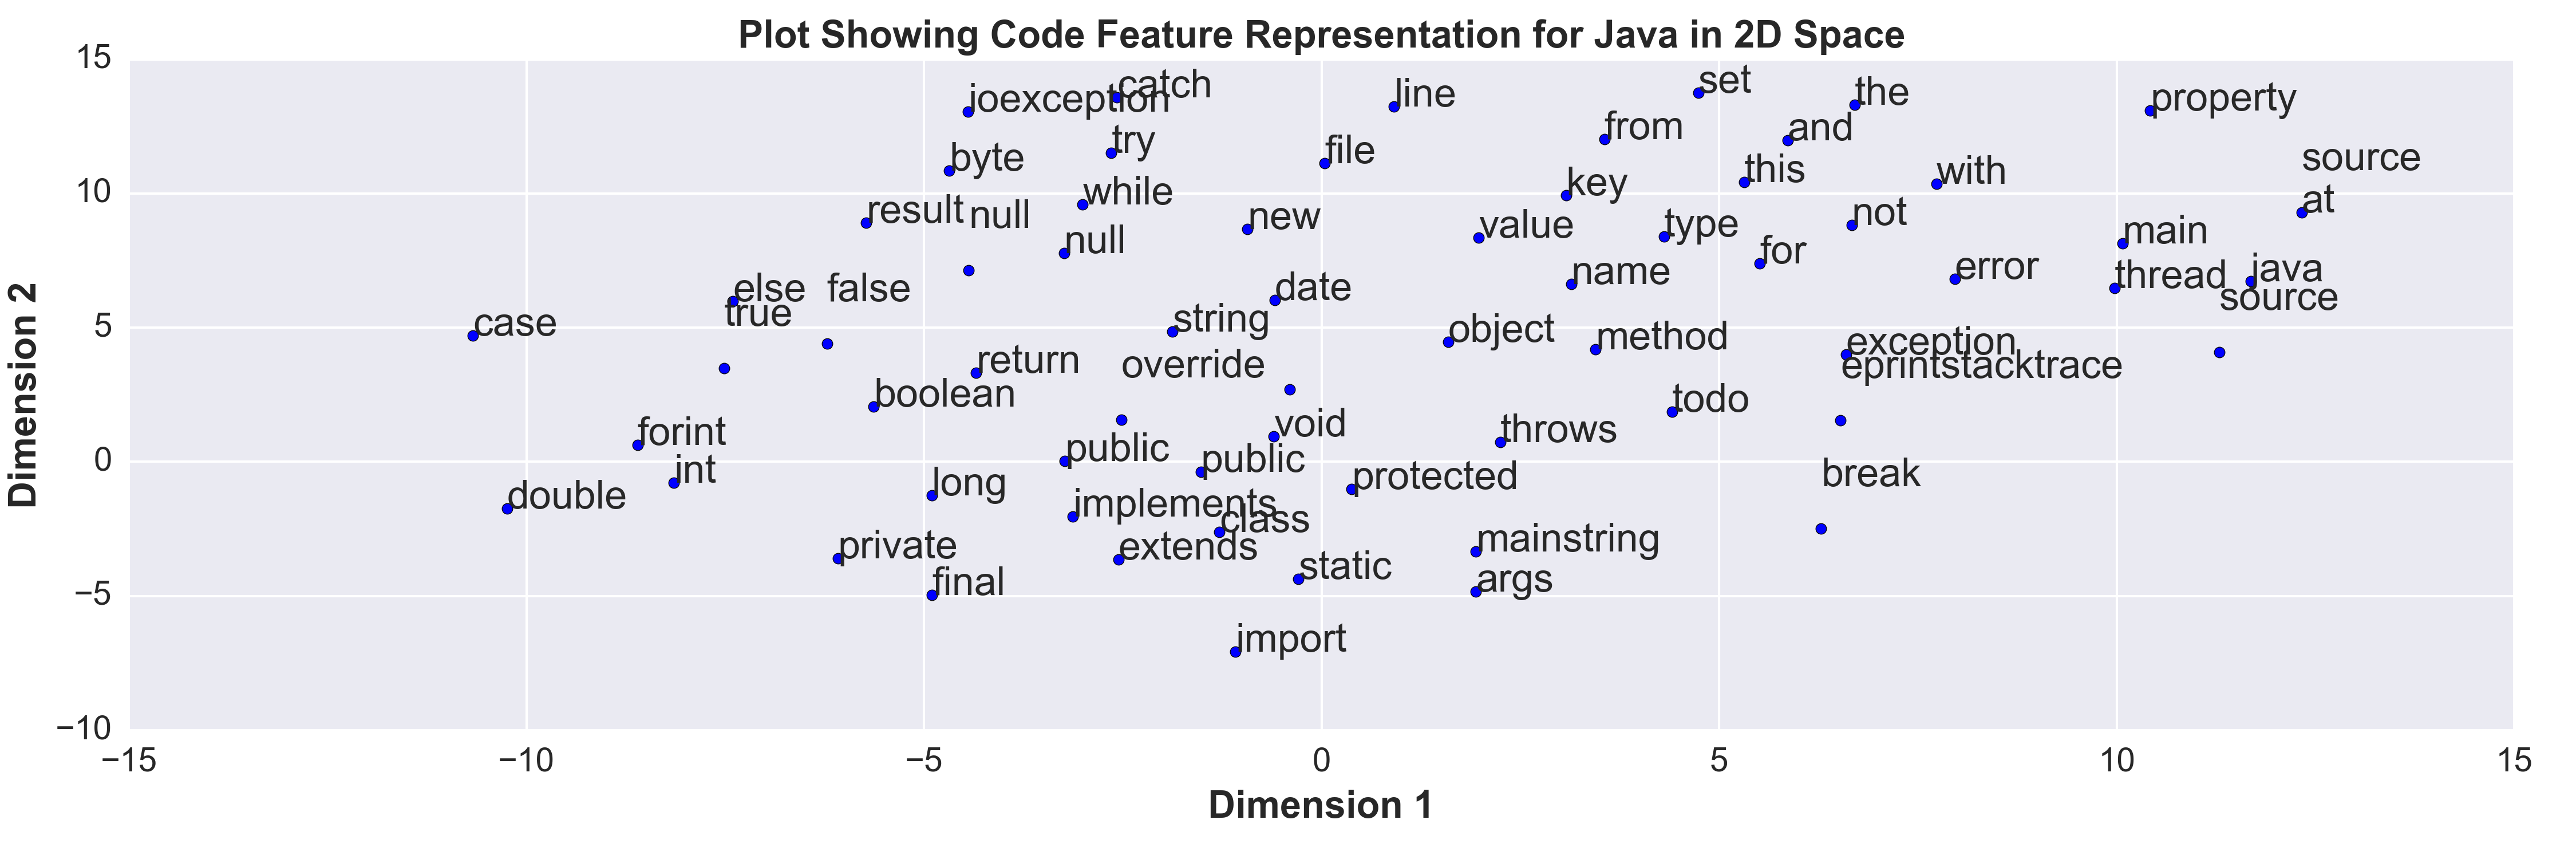
\includegraphics[width=12cm]{Fig/JavaCode} }}%
    \qquad
    \subfloat[JavaText]{{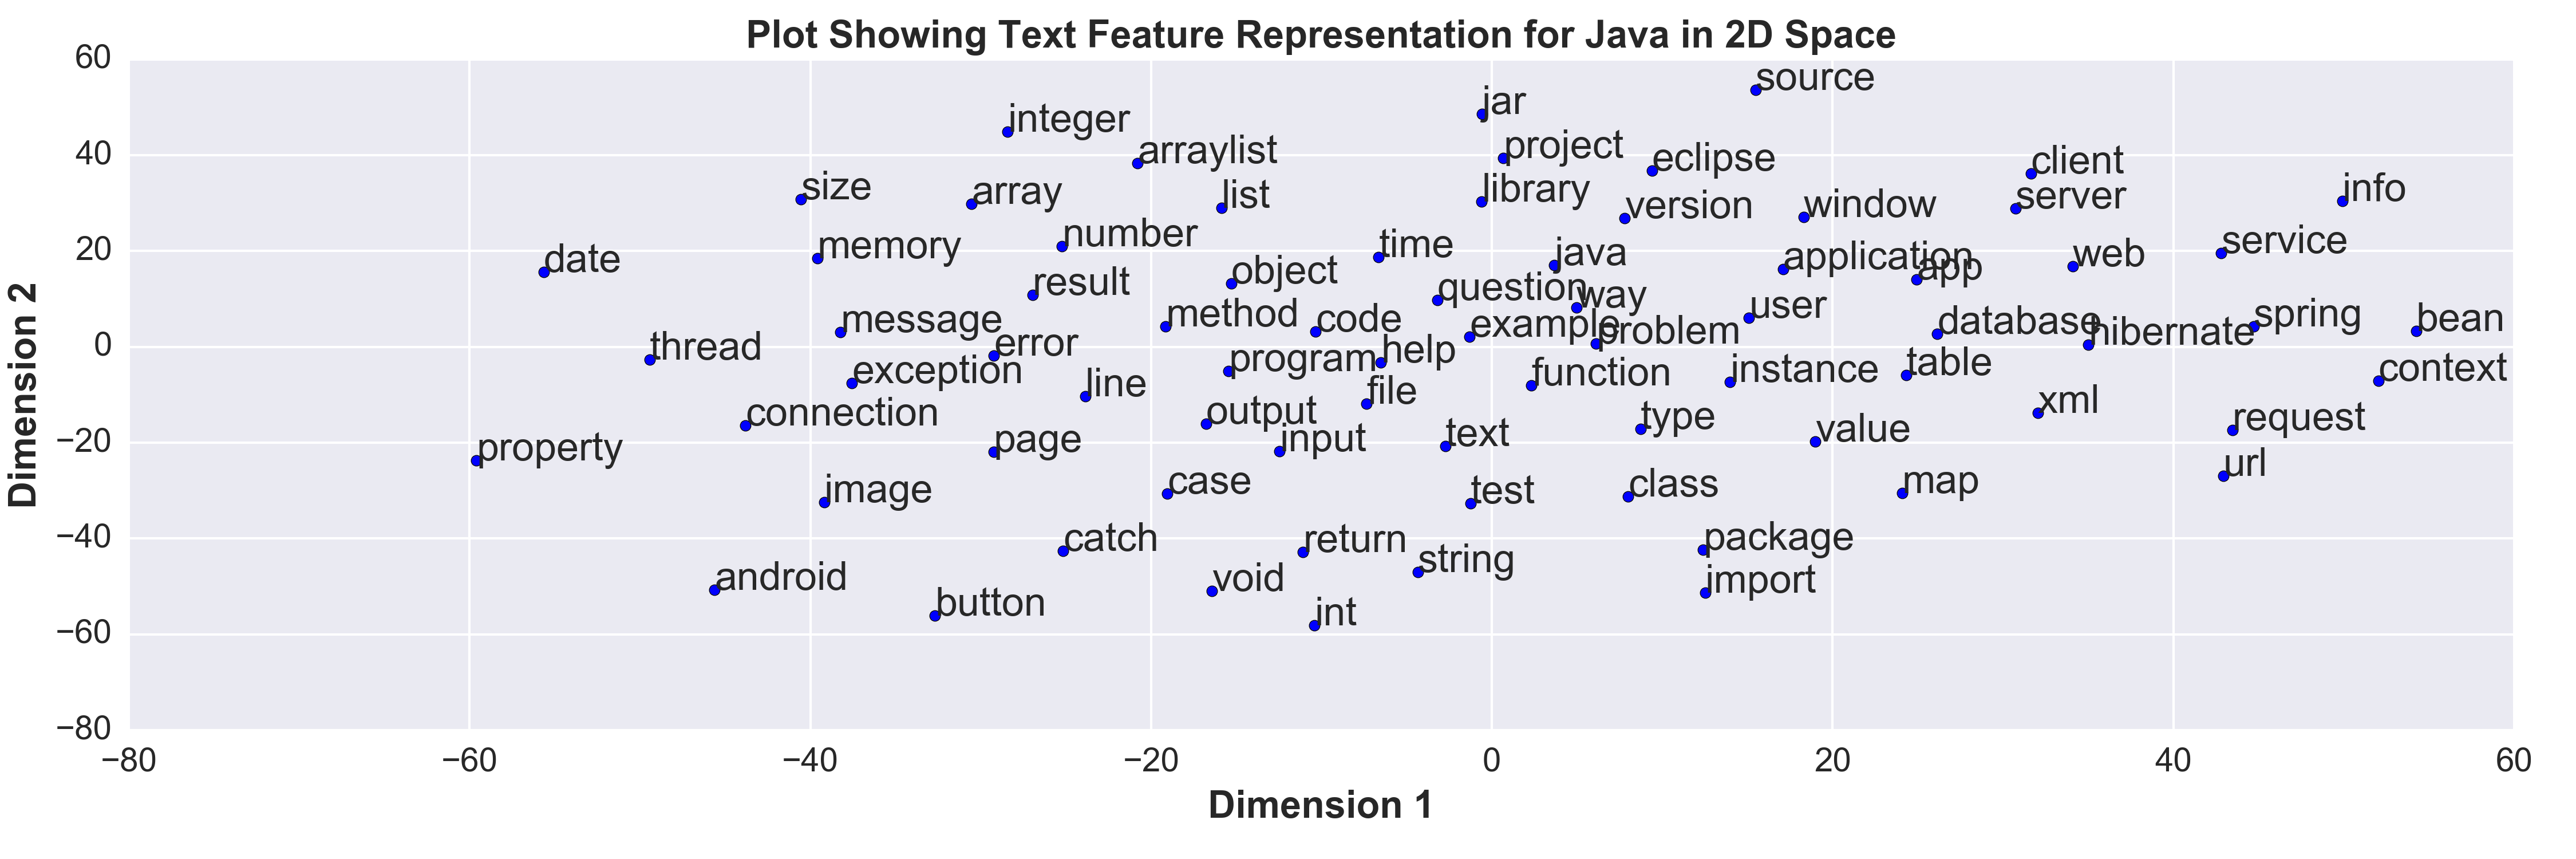
\includegraphics[width=12cm]{Fig/JavaText} }}%
    \caption{Features of Java }%
    \label{fig:Java}%
\end{figure*}
\begin{figure*}[t]
    \centering
    \subfloat[SQL Code]{{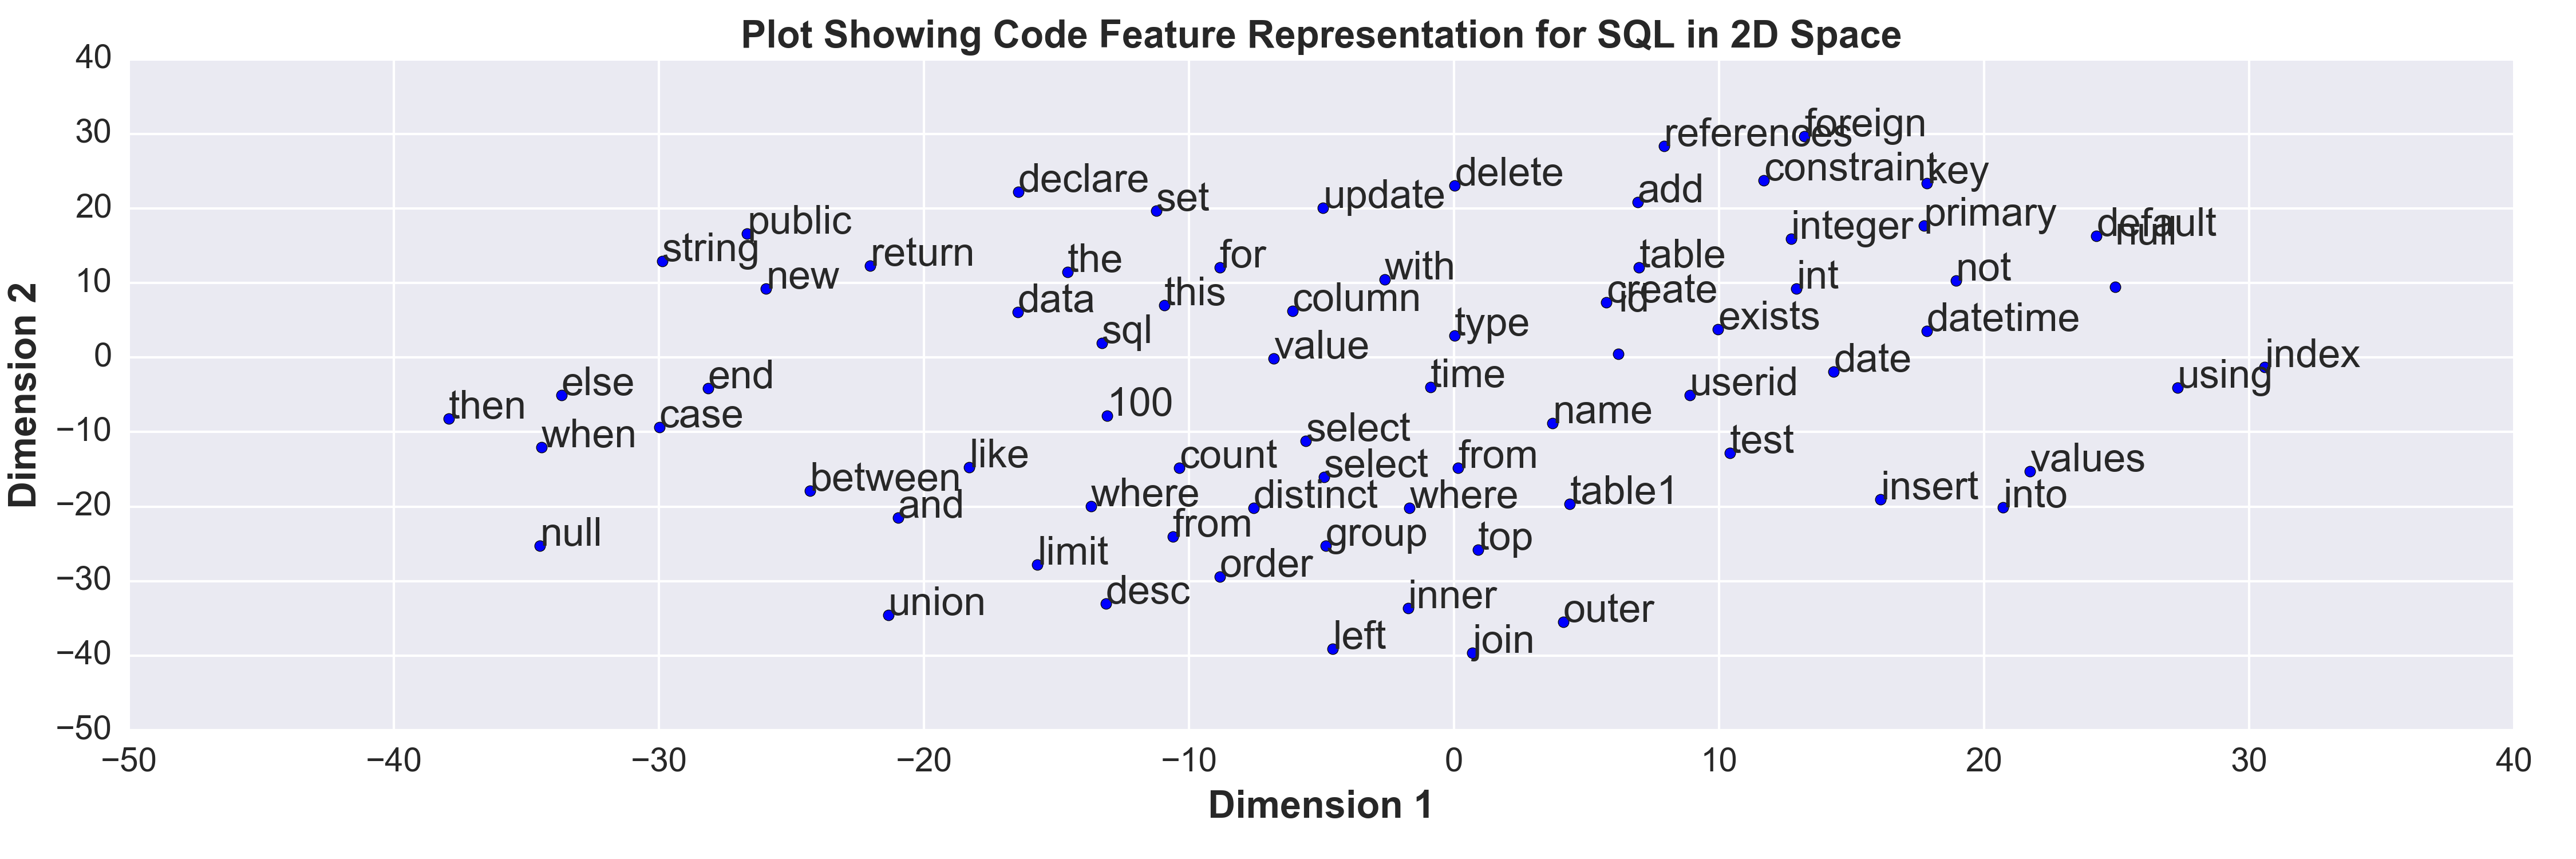
\includegraphics[width=12cm]{Fig/SQLCode} }}%
    \qquad
    \subfloat[SQL Text]{{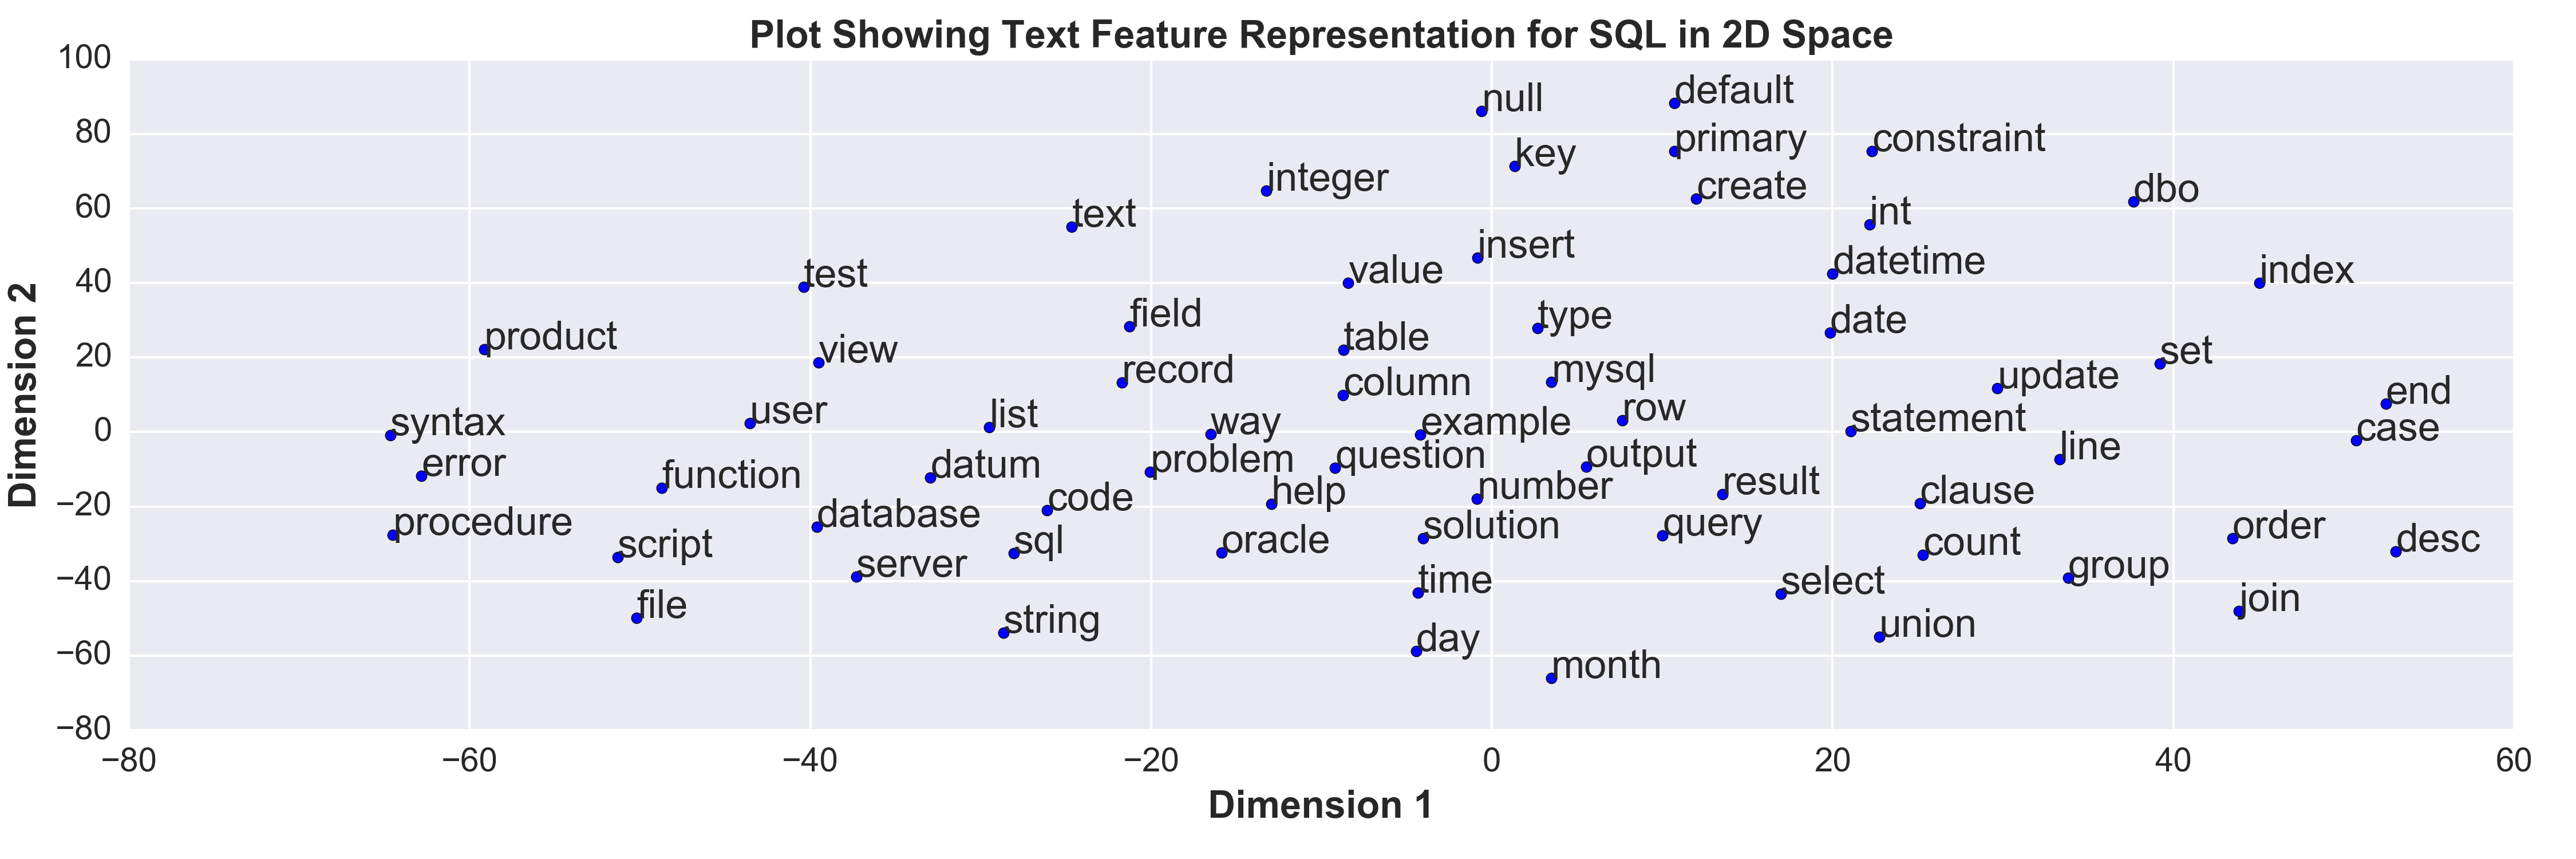
\includegraphics[width=12cm]{Fig/SQLText} }}%
    \caption{Features of SQL}%
    \label{fig:SQL}%
\end{figure*}


% second part 

\begin{res}
Can we predict the tags of programming languages by analyzing only the textual description from the data?
\end{res}
 

We trained two machine learning models (Random Forest and XGBoost) on text features extracted from Stack Overflow question. Random Forest and XGBoost achieved an accuracy of 78.4\% and 81.04\% respectively. Compared to the models trained on the code features, this is a significant improvement in performance.  The top performing languages based on F1 score metrics are Swift (0.94), Go (0.94), Coffee Script (0.93), C (0.93), Haskell (0.92), Groovy (0.91) Assembly (0.91) and Javascript (0.91).  It should be noted that Objective C performs really good when trained on text with an F1 Score of 0.90 as compared to an F1 score of 0.25 using code features. The worst performing languages are Java (0.55), C\# (0.59) and SQL (0.60). This is consistent with their performance with code features. This also implies there is not sufficient information available in the feature space (both code and text) to effectively create a good decision boundary for these languages.  It should be also noted that languages like Go, Coffee Script, Haskell, Groovy, Swift and PHP performed equally good using code and text features. 

On analysis of the feature space of top performing languages, we find that these languages have unique code features (key words/identifiers) and text features (libraries, functions). For example when we visualize the text based features for Haskell, we see words like 'GHC', 'GHCI', 'Yesod' and 'Monad'. The 'GHC', 'GHCI', are compilers for Haskell, the 'Yesod' is a web based framework and 'monad' is a functional programming paradigm (Haskell is a functional programming language). Most of top performing languages also does not have a very big feature space (Vocabulary) as compared to more popular languages like Java, Python, C\# etc which has large number of libraries, standard functions and supports multiple programming paradigms which increases the size of feature space. A large feature space adds more complexity to the machine learning models. The confusion matrix for our text feature based classifier is attached under APPENDIX A. A small number of text features that we extracted for Java and SQL could be found under Fig\ref{fig:Java} and Fig\ref{fig:SQL} respectively.


\begin{res}
Can we improve the prediction of the tags of programming languages by analyzing both the text and code snippet information from the data?
\end{res}

We combined both our text features and code features extracted from the Stack Overflow questions to train Random Forest and XGBoost classifiers. XGBoost classifier achieved an accuracy of 84.2\% where as Random Forest achieved 81.9\% accuracy on the test data. We can see that this is less than 3\% improvement over our text feature based dataset. The detailed performance metrics of our code + text combined feature classifier could be found under table \ref{Table:COdeText}. Also the confusion matrix for our top performing model could be found under Fig\ref{fig:CodeTextConf}. The performance of Java, C and C\# has improved by only 5\% by combining code and text features. There is a significant improvement in F1 Score of objective C (0.92) compared to only a score of 0.25 using code features alone. Almost all the languages except Lua, SQL, C\# and Java has both high precision and recall indicating that our machine learning model is more robust. Previous works including Baquero et al ~\cite{c18},Rekha et al ~\cite{c10} and Saha et al ~\cite{c1} all reported similar results for these languages. However, our result for these languages are significantly better both in terms of precision and recall. Combining commonly used code features (identifiers, commonly used functions etc.) and text features (library names, compiler names etc.) for languages have helped us to train better machine learning models.

The Word2Vec representations shown under Fig\ref{fig:Java} and Fig\ref{fig:SQL} were created by training splitting the code and text snippets and training their vector representations separately for each programming language. There are more than 200 feature extracted using Word2Vec for each language but we have shown only around 70 features in our figures because including a large number of features in our figures could make it obscure and unreadable. In a vector space, features which are used in the same context lies closer in the high dimensional space. For example in the Java code Fig\ref{fig:Java}, we can see that 'public','class','implements','extends' all are close to one another in vector space since they are mostly used together in a line of code. Another example we can look at is for SQL code Fig\ref{fig:SQL} where features like 'foreign', 'primary', 'key', 'constraint' and 'reference' are all used in the same context of setting relationship between tables. 

The smaller cosine distance between features doesn't mean they are used in the same line of code but used in the same context (Declaring Relationships in tables for example). Now when we look at the text features for Java we can see that this include some code features as well. This is because in Stack Overflow, people describe their issues by including code based identifiers and features along with the text not just in code blocks. However, we can also see 'netbeans', 'eclipse' which are popular IDE's for Java also present. Another key observation from the Java text feature is that 'Android' and 'spring'- a  framework for web and desktop applications are located at opposite sides of the plot(maximum cosine distance). This means that an Android developer might never use spring framework for his developmental activities. At the same time, 'spring' is located close to 'web', 'service', 'url', 'request', 'xml' etc which indicates that Spring framework is used alot in web development in Java.

The application of Word2Vec is not just for classification tasks. Training these models on both code and text features could unravel valuable insights about programming languages. This method is more robust that methods such as Latent Dirichlet Allocation (LDA) which is still popular among the software engineering community. The impressive results that we achieved in this paper could be attributed to the fact that we didn't follow a black box approach towards machine learning. But, careful analysis and visualization of features contributed more to our trained model that just machine learning. Using dependency parsing and extracting named entities using neural network techniques using Spacy helped us to reduce noise and extract import features from Stack Overflow which made a drastic difference in our performance compared to previous works. 

\begin{table*}[t]
  \centering
  \begin{tabular}{| c | c | c | c | c |}
     \hline
    Model & Description & Accuracy & Precision & Recall \\ \hline
    Algorithmia  PLI- 20 lang.& \makecell{Evaluated for 20 languages- Excluded markdown }    & 62.8\% & 68.1\% & 62.0\% \\ \hline
    Algorithmia  PLI- 17 lang.& \makecell{Evaluated for 17 languages -Excluded Bash, HTML, CSS } &   &  &\\ \hline
    Baquero [18], code snippet & \makecell{A model trained using Support Vector Machine from 18000 question posts\\ from Stack OverFlow using code features.}  & 44.6\% & 45.0\% & 44.6\% \\ \hline
     
    Baquero [18] & \makecell{A model trained using Support Vector Machine from 18000 question posts\\ from Stack OverFlow using text features}&  60.8\% & 68.1\% &  60.1\% \\ \hline
    Our classifier: code features &\makecell {XGBoost classifier trained on 17100 Stack Overflow Question posts\\ using 5000 code features}  & 62.4\% & 76.6\% & 62.4\% \\ \hline
    Our classifier: text features &\makecell {XGBoost classifier trained on 17100 Stack Overflow Question posts\\ using 5000 text features}  & 81.04\% & 82.5 & 81.4\\ \hline
    Our classifier: code and text features &\makecell {XGBoost classifier trained on 17100 Stack Overflow Question posts\\ using 10000 features}  & 84.2\%  & 85.1\% &  84.2\% \\
    \hline
  \end{tabular}
  \caption{Comparing our Model with the Previous Work.}
\end{table*}


\section{Future Work}

The study of programming language prediction from text and code snippets is still new and a lot remains to be done. Most of the existing tools focus on file extensions rather than the code itself for predicting the language. We evaluated the most popular tool Algorithmia and found it insufficient in predicting the languages. In the recent years, there have been tremendous progress made in the field of deep learning, especially time series or sequence based models such as Recurrent Neural Networks (RNN) and Long Short Term Memory (LSTM) Networks. These networks could take a sequence of text basically character by character as input and could predict the category of the sequence. We could give the source code one character at a time as input to these RNN and LSTM models and we would be able to predict the target programming language. One small draw back of this methodology is its high computational cost and it might need large Graphics Processing Unit (GPU) cluster to train and test.
 
Natural Language processing and machine learning techniques performed much better in predicting languages as compared to tools which predict from source code. Therefore, we need to ensure that additional research should be carried out to improve the results of this task. Stack Overflow texts are pretty unique in the sense they capture both the tone, sentiments and vocabulary of the developer community. There might be a variation between this vocabulary for each programming language. Therefore, it is important that we capture, understand and separate the vocabulary for each programming language. We also recommend training a Convolutional Neural Network (CNN) which are used along with Word2Vec for various NLP related tasks. CNN have shown considerable improvement in document classification tasks compared to most simple classifiers.


\section{Threats to Validity}

Construct Validity: 
In the process of creation of our data from Stack Overflow Question posts, we selected only programming language tags. However, some of the tags which are synonyms for the languages were not included in our data extraction process. For example, 'SQL SERVER', 'PLSQL', 'MICROSOFT SQL SERVER' etc are related to SQL programming language but was not included in our dataset. 

Internal validity:
We have only studied the effect of parameters such as lines of code, programming language versions on the capability of the tools. There might be other factors  which might affect the complexity of source code and in turn the accuracy of the tools. The use of dependency parsing could result in loss of important vocabulary which might affects the results of our experiments with texts. However, we have manually analyzed the vocabulary before and after the dependency parsing and other text processing steps to ensure that information related to the languages are not lost.
 
External validity: We have only used Stack Overflow as the source of data for our analysis. We have not explored other sources such as GitHub repositories. Therefore, we cannot be absolutely confident that our results would be the same across all the sources of code snippets and texts/documents on programming languages. Our research has only focused on one tool, Algorithmia, for answering our research questions. This is mainly due to the lack of availability of open source tools for predicting languages. We have tried our best to include almost all the most commonly used programming languages for our study. However, there are still more popular and powerful languages such as Cobol, Go, pascal etc which were not considered for this study.

\section{CONCLUSIONS}

In this paper we discussed the importance of predicting languages from source code and textual data. We argued that the existing tools for predicting the programming language from source code are not adequate enough considering the challenges and complexity of today's programming languages. We evaluated a tool called ProgrammingLanguageIdentification by Algorithmia market place which is a paid API service and found that it achieved only an accuracy of 62.8\% on code snippets from Stack Overflow posts. This is in direct contrast with the claimed accuracy of the tool which is 99.4\%. On analysis of the confusion matrix, we observed that some languages such as Objective C, Haskell etc. can be predicted better compared to languages such as HTML, CSS and JavaScript which are often used together.  SQL is often used as embedded code in other languages such as C, Java, C++ and python and this also affects the accuracy of the Algorithmia API which predicts language from source code.
% Talk about NLP techniques and why it provided better results.
 
Our main contribution is a method that achieves an impressive accuracy of 84.2\% by combining the code and textual features from the posts in Stack Overflow posts to predict programming languages. In contrast, we observed that using code snippet features only gives an accuracy of 62.4\% while using the textual features only provides an accuracy of 81.04\%. The use of techniques such as extraction of named entities using dependency parsing, selection of feature space using word2vec and selection of simple and highly regularized machine learning models have helped us achieve this state of the art accuracy. 

 





\addtolength{\textheight}{-12cm}   % This command serves to balance the column lengths
                                  % on the last page of the document manually. It shortens
                                  % the textheight of the last page by a suitable amount.
                                  % This command does not take effect until the next page
                                  % so it should come on the page before the last. Make
                                  % sure that you do not shorten the textheight too much.

%%%%%%%%%%%%%%%%%%%%%%%%%%%%%%%%%%%%%%%%%%%%%%%%%%%%%%%%%%%%%%%%%%%%%%%%%%%%%%%%



%%%%%%%%%%%%%%%%%%%%%%%%%%%%%%%%%%%%%%%%%%%%%%%%%%%%%%%%%%%%%%%%%%%%%%%%%%%%%%%%



%%%%%%%%%%%%%%%%%%%%%%%%%%%%%%%%%%%%%%%%%%%%%%%%%%%%%%%%%%%%%%%%%%%%%%%%%%%%%%%%
 

%\section*{ACKNOWLEDGMENT}
%Kamel Alrashedy acknowledges the financial support of the Saudi Ministry of Education through a graduate scholarship. The authors would also like to thank the Compute Canada and WestGrid Consortium for the computation resources provided for various data processing and machine learning tasks.
 


%%%%%%%%%%%%%%%%%%%%%%%%%%%%%%%%%%%%%%%%%%%%%%%%%%%%%%%%%%%%%%%%%%%%%%%%%%%%%%%%





\begin{thebibliography}{99}%page10
 
\bibitem{c1} A. K. Saha, R. K. Saha, and K. A. Schneider, “A discriminative model approach for suggesting tags automatically for stack overflow questions,” in Proceedings of the International Workshop on Mining Software Repositories. IEEE Press, 2013, pp. 73–76.
 
\bibitem{c2} C. Stanley and M. D. Byrne. "Predicting Tags for StackOverflow Posts". In
Proceedings of ICCM 2013 (12th International Conference on Cognitive Modeling), 2013.
 
\bibitem{c3} S. M. Nasehi, J. Sillito, F. Maurer, and C. Burns,"What makes a good code example? A study of programming Q\&A in StackOverflow", in Proc. ICSM, pages 25–35, 2012.
 
\bibitem{c4} J. Brandt, P. J. Guo, J. Lewenstein, M. Dontcheva, and S. R. Klemmer, “Two Studies of Opportunistic Programming: Interleaving Web Foraging, Learning, and Writing Code,” in Proceedings of CHI 2009, New York, NY, USA, 2009, pp. 1589–1598.
 
\bibitem{c5} C. Treude, O. Barzilay, and M.-A. Storey, “How Do Programmers Ask and Answer Questions on the Web?” in Proceedings of ICSE 2011, New York, NY, USA, 2011, pp. 804–807.
 
\bibitem{c6}C. McMillan, M. Grechanik, D. Poshyvanyk, Q. Xie, and C. Fu, “Portfolio: A Search Engine for Finding Functions and Their Usages,” in Proceedings of ICSE 2011, 2011, pp. 1043–1045.
 
\bibitem{c7}M. Revelle, B. Dit, and D. Poshyvanyk, “Using Data Fusion and Web Mining to Support Feature Location in Software,” in Proceedings of ICPC 2010, 2010, pp. 14–23.
 
\bibitem{c8} R. Holmes, R. J. Walker, and G. C. Murphy, “Strathcona Example Recommendation Tool,” in ACM SIGSOFT Software Engineering Notes, New York, NY, USA, 2005, pp. 237–240.
 
\bibitem{c9} B. Seaman, “The Information Gathering Strategies of Software Maintainers,” in Proceedings of ICSM 2002, 2002, pp. 141 – 149.
 
\bibitem{c10}V. S. Rekha, N. Divya, and P. S. Bagavathi. A hybrid auto-tagging system for stackoverflow forum questions. In Proceedings of the 2014 International Conference on Interdisciplinary Advances in Applied Computing, ICONIAAC ’14, pages 56:1–56:5, New York, NY, USA, 2014. ACM.
 
\bibitem{c11} Algorithmia, "ProgrammingLanguageIdentification tool", 2017. [Online]. Available: https://www.algorithmia.com.
 
\bibitem{c12}E. Loper, S. Bird, “NLTK: The natural language toolkit,” in Proc. Interact. Present. Sessions Association for Computational Linguistics, 2006, pp. 69–72.
 
\bibitem{c13}F. Pedregosa, G. Varoquaux, A. Gramfort, V. Michel, B. Thirion, O. Grisel, M.  Blondel, P. Prettenhofer, R. Weiss, V. Dubourg, J. Vanderplas, A. Passos, D. Cournapeau, M. Brucher, M. Perrot, and E. Duchesnay, “Scikit-learn: Machine learning in Python,” Journal of Machine Learning
Research, 2011.
 
\bibitem{c14}L. Mamykina, B. Manoim, M. Mittal, G. Hripcsak, and B. Hartmann, “Design Lessons from the Fastest Q\&A Site in the West,” in Proceedings of the 2011 annual conference on Human factors in computing systems, New York, NY, USA, 2011, pp. 2857–2866.


 
\bibitem{c15}M. Asaduzzaman, A. S. Mashiyat, C. K. Roy, and K. A. Schneider. "Answering questions about unanswered questions of stack overflow". In MSR, 2013.

 
\bibitem{c16} SoStats, 2017. [Online]. Available: https://sostats.github.io/last30days/

 
\bibitem{c17} Quantcast, 2017. [Online]. Available: https://www.quantcast.com
 
\bibitem{c18} J. Baquero, J. Camargo, F. Restrepo-Calle, J. Aponte, and F. Gonza ́lez, "Predicting the Programming Language: Extracting Knowledge from Stack Overflow Posts". In Advances in Computing, 2017. 
 
\bibitem{c19} R. Rehurek and P. Sojka, “Gensim–python framework for vector space modelling,” NLP Centre, Faculty of Informatics, Masaryk University, Brno, Czech Republic, 2011.
 
\bibitem{c20} T. Mikolov, I. Sutskever, K. Chen, G. S. Corrado, and J. Dean. "Distributed representations of words and phrases and their compositionality". In NIPS, pages 3111, 2013.

\bibitem{c21} L.J.P. van der Maaten and G.E. Hinton. "Visualizing data using t-SNE". Journal of Machine Learning Research, 9(Nov):2431–2456, 2008.

\bibitem{c22} Developer Survey Results 2017. [Online].  Available: https://insights.stackoverflow.com/survey/2017\#technology

\bibitem{c23} M. Honnibal and M. Johnson, “An improved non-monotonic transition system for dependency parsing,” in Proc. of the 2015 Conference on Empirical Methods in Natural Language Processing (EMNLP), 2015, pp. 1373–1378.

\end{thebibliography}

\end{document}
